\documentclass{article}
\usepackage{proof}
\usepackage{bussproofs}
\usepackage{xcolor}
\usepackage{url}
\usepackage{framed}
\usepackage{amsmath, amsfonts, amssymb}
\usepackage{mathtools}
\usepackage{cleveref}

\begin{document}
\title{Automating Interactive Theorem Provers and Certifying Automatic Theorem Provers}
\author{Arjun Viswanathan}
\date{}
\maketitle
\begin{abstract}
	Interactive theorem provers (ITPs) and automatic theorem provers (ATPs)
	are two distinct categories of theorem provers on different ends 
	of the spectrum of verifiers. On one hand, 
	ITPs are typically robust tools with a small, verified kernel, 
	making them highly reliable. However, they 
	require user intervention in the proving process, only
	offering a minimal amount of automation. ATPs, on the other hand, 
	are push-button theorem provers that use complex heuristics to prove 
	theorems; as a consequence, they have a large code-base that is hard 
	to maintain and susceptible to bugs. A lot of recent research 
	has focused on bridging the gap between these two poles 
	of theorem proving. Hammers and certified checkers 
	are tools that were born from this research, that have different 
	approaches to this problem. This work aims to 
	comprehensively study these different tools 
	with a focus on using SMT solvers as
	the ATPs enhancing automation in ITPs.
\end{abstract}

\section{Introduction}
\label{sec:intro}
	Interactive theorem provers (ITPs) or proof assistants are 
	software tools that allow formalizing of mathematical proofs.
	They provide an expressive logic to state theorems in, and 
	an interactive interface through which the user can 
	attempt to prove these theorems using methods 
	called tactics. Generally, this interface mimics a 
	written mathematical proof with a context and a goal 
	that changes on the fly as one steps through the parts 
	of the proof. The data structures provided by the ITP are 
	minimal and the user's mathematical structures are 
	defined on top of these, keeping the verified kernel of the 
	ITP small. These proofs provide a high level of reliability
	but are hard to come up with from the user's point of view. 
	
	Automatic theorem provers (ATPs) have grown rapidly over the 
	past decades and refer to tools that allow automatic proving 
	of logical formulas. Interaction between the user and the 
	ATP is kept to a minimum; ideally, the user would provide a 
	theorem to the ATP and the ATP either proves it or comes up
	with a counter-example that disproves it. ATPs are broadly divided into satisfiability modulo theories 
	(SMT)-solvers and superposition provers. Although both 
	of these have different approaches to proving, they 
	both look at a formula in terms of whether it is 
	unsatisfiable or not. The satisfiability problem 
	is the dual of the validity problem (proving a 
	formula to be valid) - a formula can be proved to be 
	valid by establishing that its negation is 
	unsatisfiable.
	
	\begin{figure}[t]
		\centering
		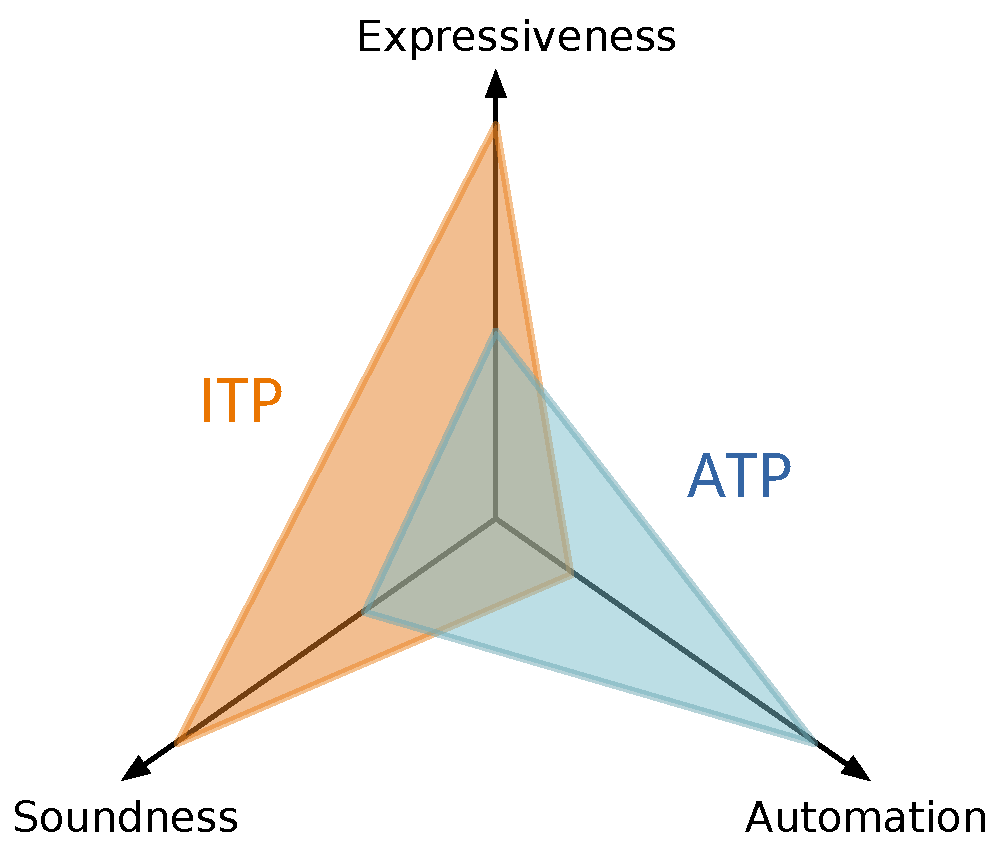
\includegraphics[scale=0.5]{coq.pdf}
		\caption{Comparing Interactive Theorem Provers (ITPs)
		and Automatic Theorem Provers (ATPs)}
		\label{fig:graph}
	\end{figure}

	ATPs and ITPs clearly have different modes of operations
	and offer distinct advantages - ITPs certify their 
	results with a high degree of trustworthiness although 
	reaching the proofs might take some time and effort from 
	the user; ATPs offer relatively quick and automated results, 
	while not giving the same kind of guarantees that ITPs do.
	A natural research question is whether we can get the best 
	of both worlds - reliable proofs with maximum automation. 
	In this work, we study various tools that 
	attempt to combine these tools. We conclude with a 
	more comprehensive study of two state-of-the-art
	integrations of SMT solvers with proof assistants -
	the \textit{smt} tactic in Sledgehammer and 
	SMTCoq. Both these tools use SMT solvers to 
	automate proofs in ITPs, but approach the 
	problem very differently. 
	two tools that take different approaches 
	to this goal. A hammer helps an ITP prove lemmas by using 
	an ATP to guide its proof search, and Sledgehammer is
	the very first of these. On the other hand, 
	a certified checker is more tightly integrated with the ATP 
	- it also converts proofs produced by the ATPs and 
	checks them within the ITP. Thus, it gets results 
	from outside the ITP but certifies them by checking them
	inside the ITP. SMTCoq is a certified checker 
	for the Coq proof assistant that uses SAT and SMT solvers
	for automation.
	
	After specifying the notation used in the rest of the 
	paper and discussing some tools in the area that 
	we don't go deep into here, we describe SMT solvers
	and superposition provers in \Cref{sec:atp}.
	\Cref{sec:itp} explores the state-of-the-art 
	of ITPs. \Cref{sec:hammer} and \Cref{sec:sledgehammer}
	explore hammers in general, and Sledgehammer's
	integration with SMT solvers in particular. In
	\Cref{sec:cert}, we look at SMTCoq, a tool that 
	takes a different approach to automating ITPs
	using SAT and SMT solvers. Finally, we compare 
	the 2 approaches in ~\Cref{sec:conc} and discuss
	our plans to take this research forward.
	\textcolor{red}{Give a preview of the rest of the paper here}

\section{Formal Preliminaries}
\label{sec:prelim}

\section{Related Work}
\label{sec:rel}
	\textcolor{red}{QED Manisfesto}\\
	\textcolor{red}{Hammer for resolution provers?}\\
	\textcolor{red}{CoqHammer}\\
	\textcolor{red}{Check related work of both papers.}\\
	\textcolor{red}{NQTHM and ACL2 are the earliest combination of ATPs and ITPs according to the SMTCoq paper}
	In ~\cite{10.1007/978-3-642-14052-5_14}, they integrate 
	Z3 with Isabelle/HOL and HOL4 
	using proof replaying, that is to verify 
	the Z3 proofs in the ITP, similar to SMTCoq. However, 
	~\cite{10.1007/978-3-642-22438-6_11} mentions that this
	integration wasn't useful. Instead, the reconstruction 
	method using the in-house Metis solver was more 
	successful. \\
	\textcolor{red}{Related work from Page 35 of Bohme's thesis}\\
	\textcolor{red}{Related work from Page 59 of Bohme's thesis}\\
	
\section{Automatic Theorem Provers}
\label{sec:atp}	
\subsection{SMT-Solvers}
\label{smt}
	Boolean satisfiability, often called the SAT problem, 
	is the problem of satisfying a Boolean formula, that is, 
	consistently assigning values of $True$ or $False$ 
	to the variables of the formula so that the entire 
	formula evaluates to $True$. For example,
	\begin{center}$(x \lor y) \land z$ \end{center}
	can be satisfied by the 
	assignment $\{x=True,\ y=False,\ z=True\}$. On the other hand, 
	\begin{center} $x \land \neg x$ \end{center}
	is unsatisfiable, no matter what value is assigned to $x$.
	
	Satisfiability Modulo Theories~\cite{DBLP:reference/mc/BarrettT18} 
	or SMT lifts SAT to a level that includes theories. 
	For example, 
	\begin{center} $(a = b) \land (b = c) \land \neg (a = c)$ 
	\end{center}
	is a formula that is unsatisfiable in the theory of 
	equality over uninterpreted functions. This is because, by
	transitivity of $a = b$ and $b = c$, we have $a = c$. SMT 
	allows us to be more expressive with our formulas, but 
	this comes at the cost of more complicated decision 
	procedures.
	
	SMT solvers have plenty of applications in formal methods 
	and software verification. For instance, SMT solvers are used 
	in the back-end of model checkers~\cite{DBLP:books/daglib/0020348}, 
	which input mathematical 
	models of a software system, and verify whether they 
	satisfy a particular property or not. Another area of 
	application is symbolic
	execution~\cite{DBLP:journals/csur/BaldoniCDDF18}, 
	which is to analyze a 
	program to figure out what set of inputs work for each 
	part of the program. Other uses of SMT solvers include 
	program synthesis~\cite{synth}, static analysis, 
	and interpolant generation~\cite{DBLP:journals/corr/abs-1111-5652}.
	
	Due to the recent emphasis on verifying results from SMT-solvers~\cite{10.1145/1670412.1670413,
	mansur2020detecting, 10.1007/978-3-642-38916-0_3},
	many SMT-solvers are proof producing. When an SMT-solver finds 
	that a formula is satisfiable, an easily checkable proof of this is 
	a satisfying model of the formula. However, when a solver 
	concludes that a formula is unsatisfiable, it is more difficult 
	to produce an acceptable proof of this. Most SMT-solvers 
	follow some version of the DPLL(T) algorithm, which tries
	to satisfy the formula by propagating assignments, making 
	choices on assignments when necessary, and concluding unsat
	when all choices have been tried. Since this algorithm 
	primarily operates on the resolution principle, 
	a universally accepted proof calculus is one based 
	on resolution. Specifically, a proof of unsatisfiability 
	of a formula in CNF, is a tree with the input 
	clauses and theory lemmas at the leaves, and the empty 
	clause at the root. The resolution rule 
	takes two clauses, a pivot element that occurs 
	with opposite polarities 
	in each of the clauses, and gives one clause that is 
	a consequent of the premises. The idea is that, beginning 
	with the input clauses and the theory lemmas (which might 
	have their own sub-proof trees coming from the theory solvers), 
	the tree derives that the empty clause holds, which is the 
	most basic notion of unsatisfiability since the there 
	is no way to satisfy the empty clause.
	
	\begin{center}
		$\infer[resolution]{\varphi_1 \lor ... \lor \varphi_n \lor 
			\psi_1 \lor ... \lor \psi_m}
		{\varphi_1 \lor ... \lor \varphi_n \lor \chi & \neg \chi 
			\lor \psi_1 \lor ... \lor \psi_m}$ 
	\end{center}
	For instance,
	\begin{center}
		$\infer{a \lor c}{a \lor \neg b & b \lor c}$
	\end{center}
	
	\begin{figure}[t]
		\fbox{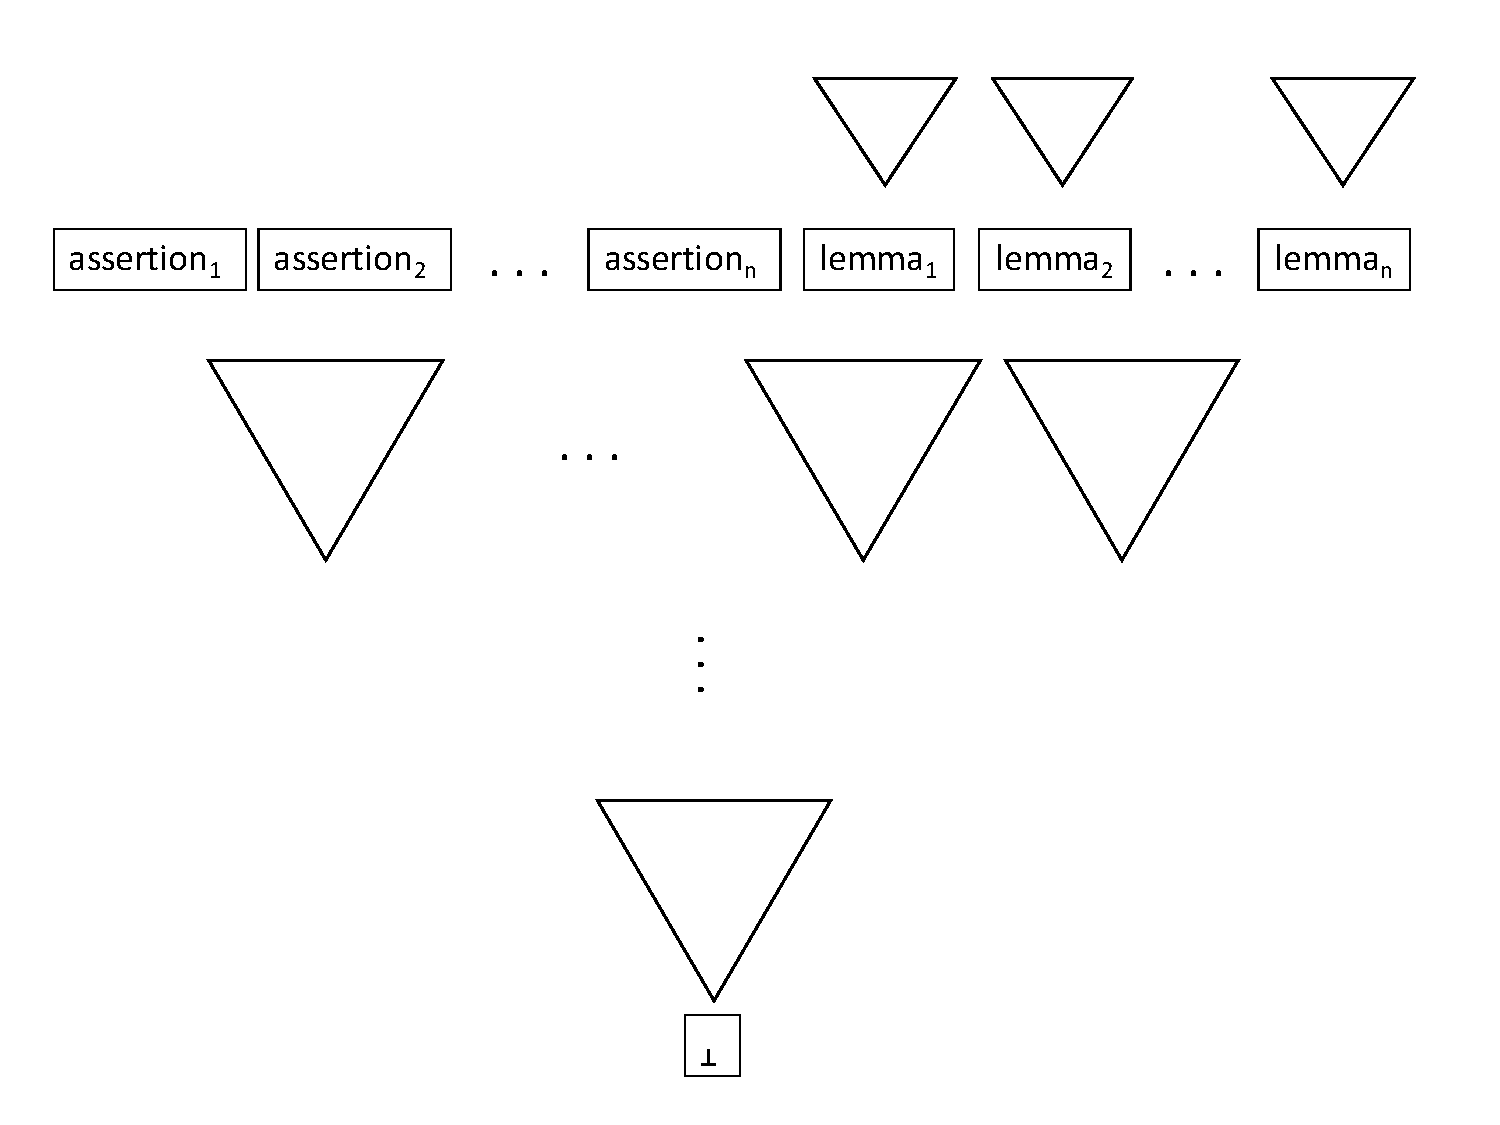
\includegraphics[scale=0.5]{prooftree.pdf}}
		\caption{A proof tree of unsatisfiability.}
		\label{fig:tree}
	\end{figure}

	The proof calculus for an SMT solver consists 
	of proof rules such as resolution and a 
	proof of unsatisfiability is a proof tree with 
	the assertions asserted in the problem as 
	leaves, as illustrated in \Cref{fig:tree}.
	Additionally, clauses asserted to 
	be true by a theory solver - called theory lemmas 
	- can also be leaves. These are usually 
	justified by the theory solver, possibly by 
	a tree rooted at the lemma. Each node in 
	the tree is an application of a proof rule, 
	and the root concludes the empty clause $\bot$.
	
	Even though the calculus is common among the SMT-solvers, 
	it hasn't been standardized. CVC4 uses a proof language called
	LFSC or (Logical Framework with Side Conditions) that mixes 
	declarative rules with computable programs; veriT uses a rule-bases 
	calculus defined in a SMTLIB like syntax; Z3 uses a rule based 
	calculus with a relatively lower level of granularity. 
	
	\subsection{Superposition Provers}
	\label{sup}
	Superposition provers or resolution provers differ 
	from SMT solvers in that they focus on proving 
	conjectures rather than finding a satisfiable model
	for a set of formulas. The problem is formulated 
	as a set of axioms that relate to the problem space, 
	a set assumptions and a conjecture to prove. 
	The goal is to find the unsatisfiability of 
	the negation of the conjecture along with the 
	assumptions and the axioms, and this is done 
	by refutation. The prover converts 
	the input formulas into a set of clauses and 
	uses a small set of inference rules to add 
	implied clauses to the input set of 
	clauses - ultimately it tries to derive 
	the empty clause or figure out that this 
	isn't possible. These provers are resolution-based -
	the most important rule in the calculus is the 
	\textit{resolution} rule. This has evolved into 
	the \textit{paramodulation} rule to accommodate 
	the notion of equality, and ultimately into 
	the \textit{superposition} rules that take into 
	consideration, along with equality, an ordering 
	on the terms in the clauses to reduce the number 
	of rule applications.
	
	At the leaves are axioms or assumptions, and 
	each node is obtained using one or more inference
	rules applied on previous nodes/leaves. 
	A proof trace is a DAG with the empty clause at
	the root. The inference rules are sound and 
	usually theoretically complete, but in practice 
	this might be only true with infinite resources.
	
	Popular resolution provers like Vampire, E, and 
	SPASS adhere to the TPTP (Thousands of Problems 
	for Theorem Provers) input/output standard.
	
	The superposition prover applies the inference 
	rules to the input set of 
	clauses until saturation - that is until the 
	resultant set of clauses is closed under the 
	inference rules. To keep this system
	efficient, provers use an ordering 
	on the terms. The saturation algorithm used 
	by the prover guides the process of adding the 
	next inference rule based on this simplification 
	ordering of terms.
	
	Given $S$, the set of input clauses, the possible 
	outcomes of a superposition prover are:
	\begin{enumerate}
		\item The empty clause is derived from $S$, and
		$S$ is unsatisfiable.
		\item The solver terminates without generating the 
		empty clause, and $S$ is satisfiable.
		\item The saturation algorithm doesn't terminate 
		before the prover runs out of resources, and 
		the empty clause isn't generated. In this 
		case, the result is unknown. 
	\end{enumerate}
	
	Since there may be redundance in the application 
	of inference rules, and the generated clauses, 
	many provers work on minimizing this redundance in 
	interest of efficiency.
	
	Resolution provers deal with theories by 
	adding an axiomatisation of the theory to the 
	leaves of the DAG before running the 
	saturation algorithm.
	
	While both SMT solvers and superposition provers 
	produce resolution proofs, SMT solvers are guided 
	by trying to find a satisfying model to an input 
	problem whereas superposition provers try 
	to prove the negation of conjecture to be unsatisfiable
	with the remaining assertions in the problem. 
	
	Additionally, theories are built-in for SMT solvers,
	while they need to be externally axiomatized for 
	resolution provers. As such, superposition provers
	are better suited for quantified formulas and 
	minimal theory reasoning, whereas SMT solvers 
	do well on problems that contain constraints 
	in theories and quantified formulas slow them 
	down.
	
\section{Proof Assistants}
\label{sec:itp}
	A proof assistant or interactive theorem prover 
	(ITP) is a software tool used for formalizing 
	of proofs by human-machine collaboration.
	Proof assistants originated with the Automath
	~\cite{10.1007/BFb0060623} and the Logic for 
	Computable Functions (LCF) theorem prover ~\cite{10.5555/891954}, which is designed 
	in the logic with the same name
	~\cite{Loeckx1987}. Both emphasized the 
	principle of having a small trustable proof 
	checker. In LCF-style theorem provers theorems 
	are implemented as an abstract datatype, and 
	new theorems can only be constructed through a 
	fixed set of functions, that correspond to the 
	underlying logic's axiom schemata and inference 
	rules, provided by this datatype. This keeps
	the trusted codebase to a minimum, and 
	provides strong soundness guarantees. These 
	include the HOL family of ITPs - HOL Light, 
	HOL4 and Isabelle. Automath is based on type 
	theory and the Curry-Howard isomorphism, where 
	propositions or theorem statements are types, 
	and their proofs are programs inhabiting them. 
	ITPs taking the Automath approach to 
	theorem-proving include Coq, Agda, NuPRL, 
	Matita, and Lean.
	
	In the following sections, we focus on 
	particular ATP integrations with Isabelle/HOL 
	and Coq. Isabelle is a proof assistant that used 
	to formalize of mathematical formulas. 
	Isabelle/HOL is an instance of Isabelle that 
	provides an expressive HOL to prove theorems in 
	its proof language Isar, and also consists of a 
	large library of formally verified mathematics. 
	The Coq proof assistant provides a functional 
	programming language interface in Gallina, and 
	implements a type theory called the calculus of 
	inductive constructions (CIC). Similar to 
	Automath, theorems are types in Coq, and 
	proofs are programs inhabiting them. While these 
	proofs are written manually by the user, Coq 
	provides some automation in the form of 
	\textit{tactics}. Using tactics, the user 
	must build a term whose type is the theorem 
	being proved, and a proof ends with 
	\texttt{Qed} which calls the Coq type checker 
	to certify the proof.	
	
\section{Hammers}
\label{sec:hammer}
	Hammers use ATPs to automate the proving of goals within ITPs
	that depend on certain other lemmas. A hammer is composed of 
	a premise selector, which is a method to identify relevant 
	premises that help prove a goal; a translator that bridges 
	the gap between the logic of the ATP and that of the ITP; 
	and a proof reconstructor that processes the ATPs proof
	within the ITP.
	
	\subsection{Premise Selection}
		While queries to SMT solvers are contained within a single 
		file, this isn't necessarily the case for ITPs. An SMT file
		typically consists along with declarations and definitions 
		of a set of assertions and a query that checks whether 
		their conjunction is satisfiable or not. 
		One can imagine a set of hypotheses 
		$H_1, H_2, ..., H_n$ and a conjecture $G$, with a 
		typical goal in an ITP that looks like $L$:
		\begin{center}
			$L : H_1 \to H_2 \to ... \to H_n \to G$.
		\end{center}
		Proving $L$ is equivalent to proving the unsatisfiability 
		of $\neg L$.
		\begin{align*}
			\neg L &= \neg (H_1 \to H_2 \to ... \to H_n \to G)\\
			&= \neg (\neg H_1 \lor \neg H_2 \lor ... \lor \neg H_n \lor G)
			& \text{by unfolding }\to \\
			&= \neg \neg H_1 \land \neg \neg H_2 \land ... \land \neg \neg H_n 
			\land \neg G
			& \text{by De Morgan's law}\\
			&= H_1 \land H_2 \land ... \land H_n \land \neg G
			& \text{by double negation elimination}
		\end{align*}
	
		So the problem can equivalently be stated in the context of ATPs
		as checking the unsatisfiability of a set of hypotheses 
		along with the negation of the conjecture. This would look 
		like the following SMT file:
		\begin{verbatim}
			assert H_1
			assert H_2
			...
			assert H_n
			assert (not G)
			check-sat
		\end{verbatim}
		However, goals in ITPs aren't necessarily self-contained 
		as in $L$. The hypotheses needed to prove $G$ 
		might have been proven earlier. In fact, ITPs have large
		libraries of proven lemmas any of which might be potentially 
		useful in proving a goal $G$. As such, picking
		the hypotheses to send along with the negation of the 
		goal to an ATP is challenging. This is called premise 
		selection. The most basic form of premise selection 
		is to allow for the user to find relevant facts 
		to prove a conjecture. But given that these libraries 
		have hundreds of lemmas, automatic methods to select 
		premises is a more scalable and generalizable approach.
	
		Historically, premise selection was delegated to the 
		user, but modern hammers have plenty of ways to 
		automate this process. Some that use machine learning
		to learn axiom selection from previously successful 
		proofs using methods such as ones based on 
		Bayesian statistics \cite{DBLP:journals/jar/AlamaHKTU14}, 
		a nearest-neighbor ranking function 
		\cite{DBLP:conf/cade/KaliszykU13a}, and non-linear 
		kernel methods \cite{DBLP:journals/jar/AlamaHKTU14}.
		Others use simpler algorithms; the relevance filter 
		by Meng and Paulson 
		\cite{DBLP:journals/japll/MengP09}
		for the Isabelle/HOL ITP selects relevant facts by 
		giving priority to the number of symbols in common 
		with the goal. The SInE (SUMO Inference Engine) 
		\cite{10.1007/978-3-642-22438-6_23} does something 
		similar in the ATP Vampire. The Divvy system 
		\cite{10.1007/978-3-642-02959-2_13} also uses a 
		syntactic relevance filtering technique but it 
		selects from the ordered facts from the middle, 
		instead of doing it from the top of the list; it
		also uses an ordering technique based 
		on latent semantics called APRILS (Automated 
		Prophesier of Relevance Incorporating Latent Semantics).
		Others use semantics instead of syntax to guide
		the selection process. For instance, the SRASS 
		(Semantic Relevance Axiom Selection System) 
		\cite{10.1007/978-3-540-73595-3_20} finds 
		countermodels of the conjecture and selects axioms that
		exclude the countermodels. Other research combined
		these various types of methods to increase efficiency 
		\cite{DBLP:journals/corr/KaliszykU13b, 
			10.1007/978-3-642-31365-3_30}.
		
		\subsection{Translation}
		ITPs allow for a more expressive higher-order logic
		(HOL) with set-theoretic notation, whereas ATPs 
		are mostly restricted to first-order logic (FOL). 
		Thus, not all 
		ITP problems are transferable to an ATP. However, 
		there is a large enough subset of problems provable
		by an ATP that can help an ITP user. When a goal is 
		provable by an ATP, it needs to be soundly translated 
		to its logic. The translation can involve various 
		tricks to eliminate higher-order constructs
		\cite{DBLP:journals/jar/MengP08} 
		such as higher order quantification, partial 
		function applications, and anonymous functions
		from the goal, and an encoding of any 
		type information where necessary. Resolution 
		provers usually don't have 
		in-built types, so a theory must be externally 
		axiomatized within the ATP. With SMT solvers, there
		maybe a stronger correspondence between some types and 
		sorts. 
	
		\subsection{Proof Reconstruction}
		Once the goal is translated to a problem understandable 
		to the ATP, the result from the ATP needs to be 
		soundly translated back to a valid ITP output.
		As previously mentioned, the validity of a goal in 
		the ITP corresponds to the unsatisfiability of its 
		negation in the ATP. If it is satisfiable, this 
		translates to a counterexample of the fact that 
		the goal holds. Hammers sometimes use ATPs 
		in this way to avoid wasting time proving 
		unprovable goals. More interestingly, if the 
		goal is found to be unsatisfiable in the ATP, 
		the refutation proof of its unsatisfiability
		needs to be consumed by the ITP. In its simplest form,
		this pipeline consists of using the ATP as an oracle, 
		that is to consider the goal to be proven in the 
		ITP if the ATP concludes that its negation is 
		unsatisfiable. This compromises the ITP's 
		trustworthiness and adds to the the trust-base, 
		the entire ATP.
		
		One way of doing this is to independently reconstruct 
		the proof in the proof assistant once the ATP finds 
		the goal to be unsatisfiable. In this case, the 
		only information the ITP gets from the ATP is that 
		the goal is provable given the premises. It does 
		not care about how the ATP proved this conjecture.
		Essentially, the ATP acts as a relevance filter for 
		the prover inside the ITP. This is done, for instance, 
		with Isabelle and the Metis prover 
		\cite{10.1007/978-3-540-74591-4_18}. A more involved
		integration involves using in addition to the premises
		the proof steps used by the ATP, as in PRocH
		\cite{10.1007/978-3-642-38574-2_18} that reconstructs 
		TPTP proofs in HOL Light.
		
\section{Sledgehammer}
\label{sec:sledgehammer}
		Sledgehammer is a component of Isabelle/HOL that uses 
	external ATPs to guide Isabelle/HOL's proving. The ATPs 
	used by Sledgehammer can be classified as resolution 
	provers and SMT-solvers. When a user wishes to 
	find a proof for a conjecture using Sledgehammer, 
	the tool picks a few hundred relevant 
	lemmas from Isabelle's libraries and sends them along 
	with the conjecture to the ATP. The conjecture is 
	translated from Isabelle's polymorphic higher-order 
	logic to the ATP's first order logic. Sledgehammer 
	runs this query parallelly by invoking all available 
	ATPs. If the ATP is able to prove the conjecture, 
	Isabelle's own prover metis sets out to reconstruct 
	this proof. Essentially, the role of the 
	ATP in this integration is to filter out relevant 
	facts for metis to efficiently work with and 
	also to eliminate disprovable sub-goals from 
	metis's search space.
	
	In the rest of this section, we expands on the work 
	done to integrate SMT-solvers with Isabelle/HOL via 
	Sledgehammer. Sledgehammer provides the \textit{smt}
	tactic to utilize this feature.
	
	This integration, like other hammer integrations, 
	consists of a premise selection phase, a translation 
	from Isabelle's HOL to the SMT solvers' FOL, and the 
	reconstruction of proofs found by the SMT solver with 
	inference rules of Isabelle/HOL. Reconstruction involves 
	either passing the minimal amount of facts needed 
	to prove the goal by the external solver to metis, 
	Sledgehammer's internal prover; or, sledgehammer 
	can construct the proof from the external prover, 
	inference by inference.	The solvers available to 
	Sledgehammer are Z3, Yices, and CVC3. Yices and CVC3 
	are trusted as oracles.	Trusting SMT solvers isn't a 
	dependable technique for previously mentioned reasons. The 
	integration with Z3 involves proof production by 
	Z3 and reconstruction of these proofs in Isabelle.
	
	\subsection{Translation}
		The integration of Sledgehammer with SMT solvers 
		consists of a translation from HOL 
		to multi-sorted FOL. The target 
		of the translation is the SMTLIB standard for 
		SMT solvers. The translation is sound - 
		validity of the translated problem implies 
		validity of the original problem - but not 
		complete - validity of the original problem 
		doesn't necessarily imply validity of the 
		translated problem. HOL is more expressive 
		than FOL. As such, all first-order terms 
		are representable in HOL. Translation of this 
		first-order subset of HOL is pretty straightforward. 
		More interestingly, the translation has to deal 
		with certain higher-order features that have 
		no obvious first-order counterpart. Some of 
		the incompleteness of the translation does 
		come from the inability to translate some 
		of these features.
		
		The type system of HOL consists 
		of type variables and compound types.
		A type variable is a schematic type that 
		can be instantiated to any particular type.
		For instance, $\alpha \to \beta$ is the type
		of all functions from some type $\alpha$ to
		some type $\beta$. This represents a 
		polymorphic type which is handled using 
		monomorphization - the process of generating
		all instances of a set of schematic terms based 
		on a set of monomorphic terms until a fixed point
		is reached. This process can be nonterminating. 
		The translation performs a fixed number of 
		monomorphization steps since the terms that 
		actually contribute to proofs are 
		typically those that are generated by the 
		first few steps. Compound types 
		are types constructed from other types - 
		$\kappa\ \tau_1 ... \tau_n$ is a type composed of 
		the types $\tau_1, ..., \tau_n$. After 
		recursively monomorphizing the types 
		$\tau_1, ..., \tau_n$, the translation 
		represents the compound type 
		$\kappa\ \tau_1 ... \tau_n$ as a first-order 
		type $\kappa^n$.
		
		Anonymous functions from HOL are translated 
		to a named function and a quantified constraint
		is added to specify the functions behavior.
		This is called $\lambda-$lifting.
		A term $t$ that contains a $\lambda-$abstraction
		(anonymous function) $\lambda x.u$ is translated 
		to a term $t$ with all occurrences of this 
		anonymous function substituted to $c$ and 
		the constraint $\forall x. c\ x = u$ is added.

		HOL also allows for partial applications of 
		functions, which are handled in the translation
		by using a constant $app$ that represents 
		explicit applications. If $c$ has arity 
		$m+1$ and is represented in the problem 
		with at least $m$ arguments, then 
		$c\ t_1 ... t_m$ is represented as is, 
		and this term can be applied to another 
		argument $t_{m+1}$ as 
		$app\ (c\ t_1 ... t_m)\ t_{m+1}$.
		
		The translation is less general than the 
		translation used by Sledgehammer for 
		superposition provers, in that, since (monomorphic) 
		types are embedded in SMT-solvers, some of the 
		types from Isabelle such as integers and reals 
		are mapped to their corresponding SMT types.
		In addition, this work was extended with 
		support for bit-vectors or machine integers
		~\cite{10.1007/978-3-642-25379-9_15}. The 
		Isabelle/HOL counterpart to the SMTLIB 
		theory of bit-vectors was developed by 
		Dawson~\cite{DAWSON200955}. All the SMTLIB
		bit-vector operations have corresponding 
		definitions in the bit-vector libraries of 
		HOL4 and Isabelle/HOL.
		
		An evaluation on this translation showed that SMT 
		solvers improved and complemented the proof automation 
		from resolution provers on many trivial and non-trivial 
		problems.
		
	\subsection{The Z3 Proof System}
		Z3's proof system is a natural deduction 
		calculus that uses 38 proof rules. Some of 
		these rules are presented in \Cref{fig:z3-rules}
		using sequents $\Gamma \vdash \varphi$ where 
		$\Gamma$ is a set of formulas called the hypotheses
		and $\varphi$ is a formula called the proposition. 
		A rule consists of one or more sequents as 
		premises and a sequent as the conclusion. A
		proof in Z3 is a directed acyclic graph (DAG)
		but we also refer to them as proof trees in
		this document. A proof tree consists of axioms 
		from the proof system as leaves, and application 
		of rules as nodes, and since proof trees 
		document unsatisfiability of the input 
		formulas, the root of the tree concludes the 
		empty clause $\bot$, which is represented by 
		the sequent $\Pi^\prime \vdash \bot$ where 
		$\Pi^\prime$ is the \textit{unsat core} - 
		a subset of the assertions $\Pi$
		initially given to Z3 to be shown unsatisfiable.
		
		\begin{figure}[t]
			\begin{equation*}
				\infer[\texttt{true}]
					{\vdash \top}
					{}
				\ \ \ \ \ 
				\infer[\texttt{asserted}]
					{\{\varphi\} \vdash \varphi}
					{\varphi \in \Pi}
				\ \ \ \ \ 
				\infer[\texttt{mp}]
					{\Gamma_1 \cup \Gamma_2 \vdash \varphi_2}
					{\Gamma_1 \vdash \varphi_1 & 
					\Gamma_2 \vdash \varphi_1 \to \varphi_2}
			\end{equation*}
			\begin{equation*}
				\infer[\texttt{hypothesis}]
				{\{\varphi\} \vdash \varphi}
				{}
				\ \ \ \ \ 
				\infer[\texttt{lemma}]
					{\Gamma \cup \{l_1,...,l_n\} \vdash \bot}
					{\Gamma \setminus \{l_1,...,l_n\} 
						\vdash \neg l_1 \lor ... \lor \neg l_n}
			\end{equation*}
			\begin{equation*}
				\infer[\texttt{iff$_\top$}]
					{\Gamma \vdash \varphi \leftrightarrow \top}
					{\Gamma \vdash \varphi}
				\ \ \ 
				\infer[\texttt{iff$_\bot$}]
					{\Gamma \vdash \varphi \leftrightarrow \bot}
					{\Gamma \vdash \neg \varphi}
				\ \ \ 
				\infer[\texttt{iff$_\sim$}]
					{\Gamma \vdash \varphi_1 \sim \varphi_2}
					{\Gamma \vdash \varphi_1 \leftrightarrow \varphi_2}
				\ \ \ 
				\infer[\texttt{refl$_\simeq$}]
					{\vdash t \simeq t}
					{}
			\end{equation*}
			\begin{equation*}
			\infer[\texttt{elim$_\land$}]
				{\Gamma \vdash l_i}
				{\Gamma \vdash l_1 \land ... \land l_n}
			\ \ \ 
			\infer[\texttt{elim$_\neg\lor$}]
				{\Gamma \vdash \neg l_i}
				{\Gamma \vdash \neg (l_1 \lor ... \lor l_n)}
			\ \ \ 
			\infer[\texttt{symm$_\simeq$}]
				{\Gamma \vdash t_2 \simeq t_1}
				{\Gamma \vdash t_1 \simeq t_2}
			\end{equation*}
			\begin{equation*}
				\infer[\texttt{trans$_\simeq$}]
					{\Gamma_1 \cup \Gamma_2 \vdash t_1 \simeq t_3}
					{\Gamma_1 \vdash t_1 \simeq t_2 & 
				 	\Gamma_2 \vdash t_2 \simeq t_3}
			 	\ \ \ \ \ 
			 	\infer[\texttt{comm$_\simeq,\approx$}]
			 		{\Gamma \vdash (t_2 \approx t_1) \simeq (t_2^{\prime} \approx t_1^{\prime})}
			 		{\Gamma \vdash (t_1 \approx t_2) \simeq (t_1^{\prime} \approx t_2^{\prime})}
			\end{equation*}
			\caption{Simple Z3 proof rules.}
			\label{fig:z3-rules}
		\end{figure}
		A representative subset of the proof rules are 
		documented in~\cite{DBLP:phd/dnb/Bohme12} and 
		some of them are repeated here to illustrate 
		the workings of the Z3 proof system. In addition
		to the simple rules from \Cref{fig:z3-rules},
		resolution is a rule that's central to the 
		proof calculus. Resolution was introduced in 
		\Cref{smt} and is a special case of it 
		called unit resolution is represented as follows in 
		the sequent calculus of Z3, where 
		$I = \{1,...,n\}$ and $J$ is a non-empty 
		subset of $I$ :\\
		\begin{equation*}
			\infer[\texttt{unit-resolution}]
				{\Gamma \cup \bigcup\limits_{j \in J}\Gamma_j \vdash \bigvee\limits_{i \in I\setminus J} l_i}
				{\Gamma \vdash \bigvee\limits_{i \in I}l_i & \langle \Gamma_j \vdash \neg l_j \rangle_{j \in J}}
		\end{equation*}
		
		Additionally, Z3 has a set of rules for converting 
		input formulas into equisatisfiable formulas in 
		conjunctive normal form (CNF) with polynomial 
		complexity, based on Tseitin's CNF conversion 
		method~\cite{Tseitin1983}. Tseitin's method 
		introduces auxiliary variables and constraints 
		asserting their equivalence with sub-formulas 
		that aren't in CNF, until the entire formula 
		is in CNF. Z3 runs this algorithm lazily and 
		optimizes it to avoid introducing too many 
		new vriables. A formula is in negation normal 
		form (NNF) if negations are applied only to
		variables and the only Boolean operators 
		in it are conjunction and disjunction. 
		NNF is an intermediate step in the CNF 
		conversion process when quantifiers are 
		involved and Z3 has a set of rules for 
		translation of formulas to NNF in linear time.
		
		The main rule for reasoning about equality 
		is the \textit{congruence} rule:
		\begin{equation*}
			\infer[\texttt{cong}]
				{\bigcup\limits_{j\in J}\Gamma_j \vdash f(t_1, ..., t_n) \simeq f(t_1^{\prime},...,t_n^{\prime})}
				{\langle \Gamma_j \vdash t_j \simeq t_j^{\prime} \rangle_{j \in J} & 
				\langle t_i \equiv t_i^{\prime} \rangle_{i \in I\setminus J}}
		\end{equation*}
		Equality ($=$), equivalence ($\iff$), and 
		equisatisfiability ($\sim$) are congruence 
		relations, and $\simeq$ represents any one 
		of these relations. $I$ and $J$ are defined 
		as above for resolution.
		
		Z3 is also proof producing for quantified formulas.
		$Q$ represents either of the two quantifiers - 
		the universal quantifier $\forall$ or the 
		existential quantifier $\exists$ - and 
		$\overline{x}$ represents a lost of variables 
		$x_1,...,x_n$. The following 
		proof rule allows introduction of quantifiers:
		\begin{equation*}
			\infer[\texttt{intro$_Q$}]
			{\Gamma \vdash (Q \overline{x}.\varphi_1 [ \overline{x}]) \sim (Q \overline{x}.\varphi_2 [ \overline{x}])}
			{\Gamma \vdash \varphi_1 [\overline{x}] \sim \varphi_2 [\overline{x}]}
		\end{equation*}
		The universal quantifier can be eliminated by 
		instantiation and an existential quantifiers 
		can be eliminated using skolemization.
		\begin{equation*}
		\infer[\texttt{inst$_\forall$}]
			{\neg(\forall\overline{x}.\varphi[\overline{x}])
			\lor \varphi[\overline{x} \mapsto \overline{t}]}
			{}
		\end{equation*}
		Skolemization~\cite{NONNENGART2001335} is the process 
		of removing existential quantifiers from formulas using 
		constants called Skolem constants as witnesses.
		\begin{equation*}
		\infer[\texttt{sk$_\exists$}]
			{(\exists\overline{x}.\varphi[\overline{y},\overline{x}]) 
			\sim \varphi[\overline{y},\overline{f}(\overline{y})]}
			{}\ \ \ \ 
		\infer[\texttt{sk$_\forall$}]
		{(\neg\forall\overline{x}.\varphi[\overline{y},\overline{x}]) 
			\sim (\neg \varphi[\overline{y},\overline{f}(\overline{y})])}
		{}	
		\end{equation*}
		
		Besides these, Z3 provides theory rules, 
		that conclude disjunctions of theory literals 
		called theory lemmas, for theory specific reasoning
		and rewriting rules. These are called 
		\texttt{th-lemma} rules. The theory of bit-vectors
		has special \texttt{th-lemma-bv} rules owing to 
		the fact that bit-vector proofs involve reasoning 
		about the corresponding bits of a bit-vector - 
		a process called bit-blasting. Rewriting is an 
		important part of SMT solvers - this process takes 
		care of various simplifications and 
		transformations to canonical forms. Z3 
		provides a set of metatheorems that are 
		rewriting patterns that may repeatedly 
		occur such as symmetry of equality, common 
		propositional tautologies, etc. Sledgehammer
		allows users to add rules to the set of 
		metatheorems. If one of Z3's rewrite rules 
		fails to be reconstructed in Sledgehammer, 
		the user can add a metatheorem that 
		matches the pattern to fix the failure.
		For the bit-vector 
		extension~\cite{10.1007/978-3-642-25379-9_15}, 
		schematic theorems that play the same roles 
		as metatheorems - if a theorem's conclusion 
		matches a term, the entire theorem is 
		instantiated by the scheme - proved to 
		be crucially time-saving. Besides commutativity 
		and associativity rules specific to bit-vector
		operations, examples include simplification 
		rules such as neatrality of the bit-vector 
		representing $0$ for bit-wise disjunction.
		
	\subsection{Proof Reconstruction}
		The \textit{smt} tactic trusts the Yices 
		and CVC3 solvers, so only proofs produced 
		by Z3 are reconstructed in Isabelle.
		The Z3 proofs are reconstructed step-by-step,
		and currently supported theories are equality, 
		linear arithmetic, and bit-vector arithmetic.
		Since Z3's FOL is a subset of Isabelle's HOL,
		formulas in Z3 proofs are easily representable 
		as terms in Isabelle/HOL. The Z3 proof tree
		is scanned in depth-first post-order, starting 
		from the root node, and reconstructed in Isabelle,
		step-by-step. Each proof node, contains information 
		such as rule name, references to premises and 
		propositions, and is represented as an 
		algebraic datatype with a unique ID assigned
		by Z3. Sledgehammer stores these in a balanced 
		tree with logarithmic lookup using the IDs as
		keys. Reconstruction of a proof node 
		represents a proven Isabelle/HOL theorem of 
		the node's conclusion. Every node's 
		premises are discharged as theorems, which are then 
		used to derive the node's conclusion. Once 
		reconstructed, a proof node can be reused 
		by Sledgehammer. If $\Pi$ is the set of asserted 
		formulas, $\Pi^\prime$ represents the unsat 
		core returned by Z3 - the minimal subset of 
		$\Pi$ required to prove the problem unsat. 
		After reconstructing the root node, Sledgehammer 
		checks the rest of the tree to see that only the 
		formulas from $\Pi^\prime$ remain as leaves.
		
		Proof reconstruction is sound by construction 
		and doesn't extend the trusted code base
		beyond Isabelle's LCF kernel, but incomplete. 
		In fact, this integration discovered soundness
		bugs in Z3 that were subsequently fixed by the 
		developers.
		
		For the theory of bit-vectors, the \textit{smt}
		tactic involves some additional optimizations 
		to offset the complexity added by bit-blasting - 
		a process that can cause exponential blow-up. 
		One of these - schematic theorem instantiation - 
		is described in the previous sub-section. 
		Memoization of theorems, that is, caching of 
		certain computationally expensive bit-vector 
		specific theorems in a structure called a term net 
		also proved useful. These techniques, and many 
		useful bit-vector rewrite rules - are used 
		with HOL4 and Isabelle/HOL's existing automation
		for bit-vector reasoning.
		
		Since Z3's proofs are relatively coarse-grained
		proof reconstruction in Sledgehammer has to perform
		proof search when the proof step isn't reflected 
		in Z3's proof. The author's claim that this is 
		a potential for improvement of the integration.
		
\section{SMTCoq}
\label{sec:cert}
	SMTCoq implements a skeptical cooperation between 
	Coq and proof-producing SAT and SMT solvers. 
	It can be used as a proof checker for proofs 
	produced by SAT and SMT solvers. More relevantly, 
	it is a Coq plugin that uses SAT and SMT solvers to 
	prove goals in Coq. It is written and proved 
	correct in Coq, with some OCaml support for 
	translation and preprocessing. SMTCoq allows 
	the user to query a number of SAT/SMT solvers 
	and if the solver is able to validate the query, 
	that is, it determines that the negation of the 
	conjecture is unsatisfiable, it produces a proof 
	of unsatisfiability, which is checked in Coq.
	
	Since different SMT solvers produce resolution 
	proofs of unsatisfiability in different formats, 
	SMTCoq has its own input certificate format. 
	The proofs from the different SMT solvers are 
	translated to an SMTCoq certificate which 
	can then be checked within Coq. Given an input 
	query, the SMT solver first converts into CNF
	(conjunction normal form) which is better 
	suited for resolution proofs. The proof is a 
	resolution proof which might consist of smaller proofs 
	of theory lemmas from the theory solver. 
	
	\begin{figure}[t]
		\centering
		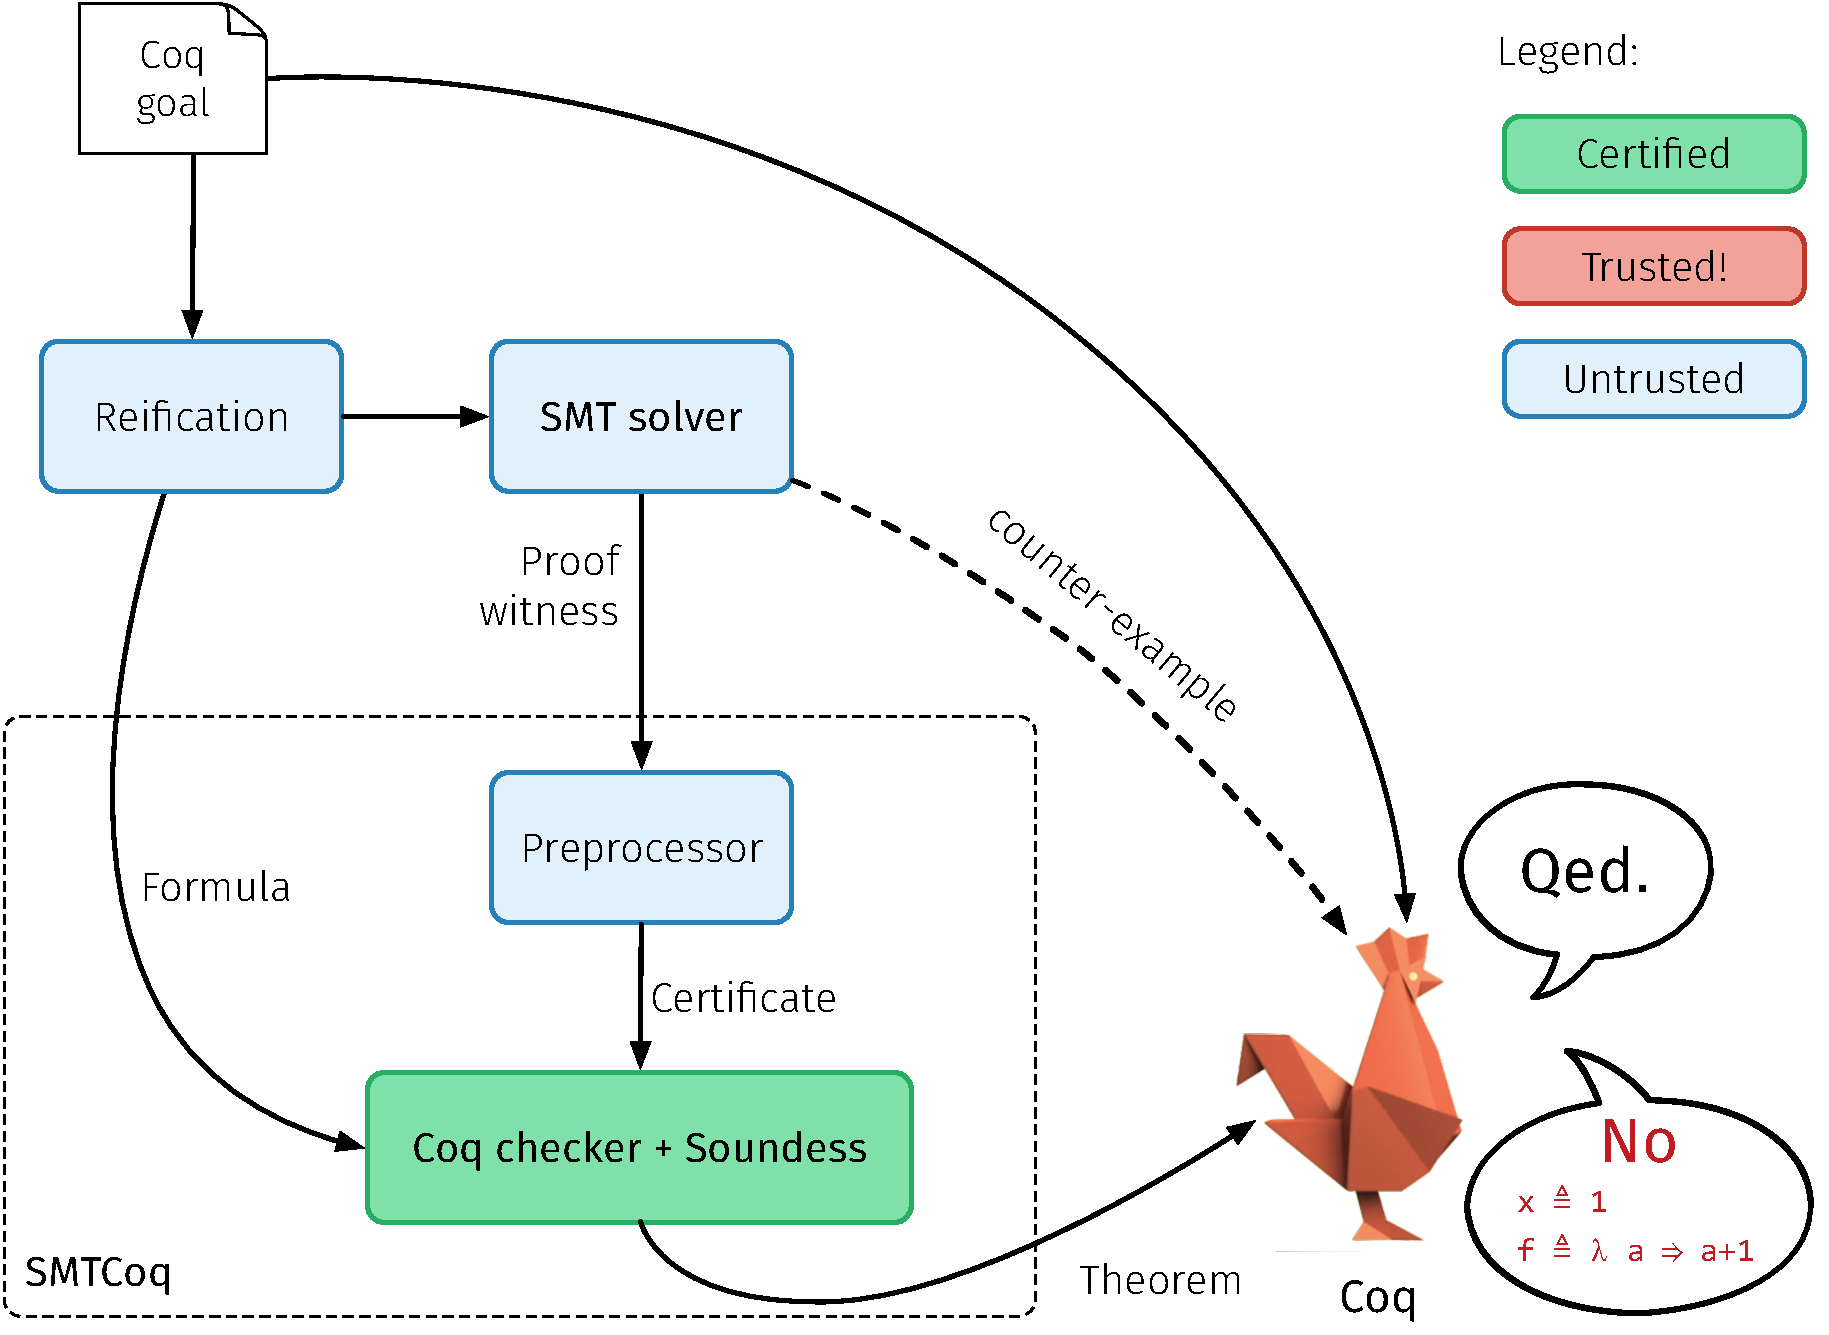
\includegraphics[scale=0.4]{tactic_cex.pdf}
		\caption{SMTCoq's integration with SMT solvers.}
		\label{fig:smtcoq}
	\end{figure}
	
	
	SMTCoq takes a modular approach of checking this proof.
	The checker is divided into a main checker that 
	delegates parts of the proof to small checkers. The proof 
	is divided into steps that small checkers can check.
	There is a small checker each for CNF conversion, 
	resolution, and for each theory. The main checker divides the 
	proof into steps, gives the step to the relevant small 
	checker, and checks that in the end, the empty 
	clause is deduced from the initial query. Each small 
	checker operates independently and maintains an invariant
	that allows the checking process to be split this way.
	
	Currently SMTCoq supports the SAT solvers zChaff and Glucose, 
	and the SMT solvers CVC4 and veriT. 
	
	SMTCoq uses Coq's native arrays to store the clauses, 
	a set of which represent the goal. The main checker 
	handles this initial array of clauses representing the 
	goal in CNF, and each small checker computes a 
	clause that is implied from a subset of the clauses.
	For efficiency, SMTCoq replaces the unnecessary 
	clauses with new ones when it knows that they 
	wont be useful anymore. After all the steps 
	are handled by the small checkers, the main 
	checker checks that the final implied clause is 
	the empty clause.
	
	\textcolor{red}{Deep vs shallow embedding}\\
	\textcolor{red}{Reification}\\
	\textcolor{red}{Important lemmas - the one that equates the embeddings}\\
	
\section{Comparison}
\label{sec:comp}
	Sledgehammer has 3 possible integrations with SMT solvers - 
	it either trusts the SMT solver as an oracle; it uses the 
	SMT solver as a relevance filter on premises so it can 
	prove goals efficiently using metis; it reconstructs 
	proofs produced by the SMT solver to produce goals 
	without compromising the soundness guarantees of the 
	small LCF-kernel. The third of these is most comparable 
	to how SMTCoq operates - it sends Coq conjectures to the 
	SAT or SMT solver, which returns a proof of the conjecture 
	if it finds it to be provable; SMTCoq then checks this 
	proof within Coq by reflection. SMTCoq can also be used as a 
	checker for proofs produced by SMT solvers. In fact, while 
	there exists an independent LFSC checker for LFSC proofs 
	provided by CVC4, veriT, while proof producing, doesn't 
	have a dedicated checker. It relies on integrations with 
	proof assistants to check its output. In this section, we 
	compare the usage of SMTCoq and Sledgehammer in their 
	capacity to use SMT solvers to automated proofs within 
	their respective ITPs.
	
	ITPs have more expressive logics than ATPs. Roughly, the 
	logic of an ATP is a subset of that of an ITP. So they 
	can be used to automate goals that are expressed within 
	this subset. Sledgehammer goes a little further by 
	describing a translation of certain HOL features 
	into FOL features understood by SMT solvers. While this 
	translation is incomplete, it captures enough HOL features 
	to widen the set of problems that an SMT solver can 
	help automate. As a consequence SMTCoq's tactics 
	cannot be called on Coq goals that contain anonymous 
	functions or partial function applications. 
	SMTCoq doesn't deal with polymorphic types 
	or compound types either. There is a correspondence between 
	types in Coq and theories in SMT, and only Coq 
	goals that have these particular types can use the 
	SMT solver. The integer sort from SMTLIB is mapped to Coq's 
	$Z$ type, and Coq's $Bool$ type corresponds to propositional 
	reasoning in SAT or SMT. However, SMTCoq defines custom types 
	for machine integers and arrays. While these serve as rich,
	independent Coq libraries for these types, they are 
	not standardized in Coq. On the contrary, Sledgehammer 
	only supports the theories of linear integer arithmetic
	and bit-vectors, besides equality over uninterpreted functions
	which both Sledgehammer and SMTCoq have support for. 
	Additionally, SMTCoq doesn't have support for quantified 
	formulas. Although the goal in Coq is universally 
	quantified, on the SMT side, it amounts to checking the 
	unsatisfiability of a quantifier-free formula. This is not 
	the case with formulas containing either alternating 
	quantifiers, or those that occur outside the head of the 
	formula - SMTCoq will fail on these. Sledgehammer uses 
	Z3's quantifier proofs to support quantified fragments of 
	its theories.
	
	Premise selection is a crucial part of Sledgehammer. A lot 
	of research has gone into optimizing premise selection to 
	make proving more efficient. Consequently, the SMT 
	integration also uses Sledgehammer's premise selection 
	mechanisms to supply the SMT solver with the best 
	possible hypotheses to prove a goal. This process is 
	so imperative that using the SMT solver just as a 
	relevance filter for premises has given useful 
	results. In SMTCoq, each lemma is considered an 
	independent entity with its set of hypotheses $H$ and 
	goal $G$ that are translated to an SMTLIB problem. 
	If the proof of $G$ depends on conjectures stated
	outside of $H$, the SMT solver will likely not be 
	able to prove them. This difference in 
	ideology comes from the difference in axiomatizations
	of theories in SMT solvers and resolution provers. 
	Sledgehammer was originally coupled only 
	with resolution provers that don't have notions of 
	theories. Any additional axioms of a theory 
	must be appended to the input of a superposition 
	prover. SMT solvers have theories encoded into them, 
	which might have facts besides $H$ that might help 
	prove $G$. However, this might not always be the case.
	We propose an extension to SMTCoq using abduction 
	to deal with this shortcoming.
	
	The Sledgehammer integration with SMT solvers is 
	specific to Z3 (although there are looser integrations 
	with other SMT solvers). Although SMT solvers have 
	a common input/output syntax in SMTLIB, their 
	proof formats are quite different. Extending 
	Sledgehammer's \textit{smt} tactic to other 
	SMT solvers might not be straightforward due to 
	the idiosyncrasies of Z3. On the other hand, SMTCoq
	claims to be generic and extensible. SMTCoq has a 
	certificate format, that is different from the proof 
	formats of each SMT solver. To extend SMTCoq's 
	support with a new solver, one only needs to 
	write a preprocessor that translates proofs from 
	this solver's format to that of the SMTCoq certificate.
	The SMTCoq checker's soundness lemmas are also generic 
	enough to add more theories simply by extending 
	the type of terms in SMTCoq. These claims are reinforced
	by extensions to SMTCoq. Initially, it had support only 
	for the ZChaff SAT solver and the veriT SMT solver, 
	with the ability to reason in the theories of EUF and 
	LIA. Since its inception, the CVC4 SMT solver and 
	the theories of bit-vectors and arrays have been 
	added to SMTCoq's capabilities.
	
	\textcolor{red}{evaluation?}
	
\section{Conclusion and Moving Forward}
\label{sec:conc}

\bibliographystyle{abbrv}
\bibliography{bib}

\end{document}